\documentclass[12pt, oneside]{article}

\usepackage[letterpaper, scale=0.8, centering]{geometry}
\usepackage{fancyhdr}
\setlength{\parindent}{0em}
\setlength{\parskip}{1em}

\pagestyle{fancy}
\fancyhf{}
\renewcommand{\headrulewidth}{0pt}
\rfoot{{\footnotesize Copyright Daniel Grier / Mia Minnes, 2023, Version \today~(\thepage)}}

\usepackage{titlesec}

\author{CSE105Sp23}

\newcommand{\instructions}{{\bf For all HW assignments:} Weekly homework 
may be done individually or in groups of up to 3 students. 
You may switch HW partners for different HW assignments. 
The lowest HW score will not be included in your overall HW average. 
Please ensure your name(s) and PID(s) are clearly visible on the first page of your homework submission 
and then upload the PDF to Gradescope. If working in a group, submit only one submission per group: 
one partner uploads the submission through their Gradescope account and then adds the other group member(s) 
to the Gradescope submission by selecting their name(s) in the ``Add Group Members" dialog box. 
You will need to re-add your group member(s) every time you resubmit a new version of your assignment.
 Each homework question will be graded either for correctness (including clear and precise explanations and 
 justifications of all answers) or fair effort completeness. You may only collaborate on HW with CSE 105 students 
 in your group; if your group has questions about a HW problem, you may ask in drop-in help hours or post a private 
 post (visible only to the Instructors) on Piazza.

All submitted homework for this class must be typed. 
You can use a word processing editor if you like (Microsoft Word, Open Office, Notepad, Vim, Google Docs, etc.) 
but you might find it useful to take this opportunity to learn LaTeX. 
LaTeX is a markup language used widely in computer science and mathematics. 
The homework assignments are typed using LaTeX and you can use the source files 
as templates for typesetting your solutions.
To generate state diagrams of machines, we recommend using Flap.js
or JFLAP. Photographs of clearly hand-drawn diagrams may also be used. We recommend that you
submit early drafts to Gradescope so that in case of any technical difficulties, at least some of your
work is present. You may update your submission as many times as you'd like up to the deadline.


{\bf Integrity reminders}
\begin{itemize}
\item Problems should be solved together, not divided up between the partners. The homework is
designed to give you practice with the main concepts and techniques of the course, 
while getting to know and learn from your classmates.
\item You may not collaborate on homework with anyone other than your group members.
You may ask questions about the homework in office hours (of the instructor, TAs, and/or tutors) and 
on Piazza (as private notes viewable only to the Instructors).  
You \emph{cannot} use any online resources about the course content other than the class material 
from this quarter -- this is primarily to ensure that we all use consistent notation and
definitions (aligned with the textbook) and also to protect the learning experience you will have when
the `aha' moments of solving the problem authentically happen.
\item Do not share written solutions or partial solutions for homework with 
other students in the class who are not in your group. Doing so would dilute their learning 
experience and detract from their success in the class.
\end{itemize}

}

\newcommand{\gradeCorrect}{({\it Graded for correctness}) }
\newcommand{\gradeCorrectFirst}{\gradeCorrect\footnote{This means your solution 
will be evaluated not only on the correctness of your answers, but on your ability
to present your ideas clearly and logically. You should explain how you 
arrived at your conclusions, using
mathematically sound reasoning. Whether you use formal proof techniques or 
write a more informal argument
for why something is true, your answers should always be well-supported. 
Your goal should be to convince the
reader that your results and methods are sound.} }
\newcommand{\gradeComplete}{({\it Graded for completeness}) }
\newcommand{\gradeCompleteFirst}{\gradeComplete\footnote{This means you will 
get full credit so long as your submission demonstrates honest effort to 
answer the question. You will not be penalized for incorrect answers. 
To demonstrate your honest effort in answering the question, we ask 
that you include your attempt to answer *each* part of the question. 
If you get stuck with your attempt, you can still demonstrate 
your effort by explaining where you got stuck and what 
you did to try to get unstuck.} }

\usepackage{tikz}
\usetikzlibrary{automata,positioning,arrows}

\usepackage{amssymb,amsmath,pifont,amsfonts,comment,enumerate,enumitem}
\usepackage{currfile,xstring,hyperref,tabularx,graphicx,wasysym}
\usepackage[labelformat=empty]{caption}
\usepackage[dvipsnames,table]{xcolor}
\usepackage{multicol,multirow,array,listings,tabularx,lastpage,textcomp,booktabs}

% NOTE(joe): This environment is credit @pnpo (https://tex.stackexchange.com/a/218450)
\lstnewenvironment{algorithm}[1][] %defines the algorithm listing environment
{   
    \lstset{ %this is the stype
        mathescape=true,
        frame=tB,
        numbers=left, 
        numberstyle=\tiny,
        basicstyle=\rmfamily\scriptsize, 
        keywordstyle=\color{black}\bfseries,
        keywords={,procedure, div, for, to, input, output, return, datatype, function, in, if, else, foreach, while, begin, end, }
        numbers=left,
        xleftmargin=.04\textwidth,
        #1
    }
}
{}
\lstnewenvironment{java}[1][]
{   
    \lstset{
        language=java,
        mathescape=true,
        frame=tB,
        numbers=left, 
        numberstyle=\tiny,
        basicstyle=\ttfamily\scriptsize, 
        keywordstyle=\color{black}\bfseries,
        keywords={, int, double, for, return, if, else, while, }
        numbers=left,
        xleftmargin=.04\textwidth,
        #1
    }
}
{}

\newcommand\abs[1]{\lvert~#1~\rvert}
\newcommand{\st}{\mid}

\newcommand{\A}[0]{\texttt{A}}
\newcommand{\C}[0]{\texttt{C}}
\newcommand{\G}[0]{\texttt{G}}
\newcommand{\U}[0]{\texttt{U}}

\newcommand{\cmark}{\ding{51}}
\newcommand{\xmark}{\ding{55}}


\newcommand{\SUBSTRING}{\textsc{Substring}}
\newcommand{\REP}{\textsc{Rep}}
\newcommand{\blank}{\scalebox{1.5}{\textvisiblespace}}


\title{HW1 : Regular Expressions and Finite Automata}
\date{Due: April 11th at 5pm (no penalty late submission until 8am next morning), via Gradescope}


\begin{document}
\maketitle
\thispagestyle{fancy}


{\bf In this assignment,}

You will practice reading and
applying the definitions of alphabets, strings, languages, Kleene star, and regular expressions.
You will use regular expressions and relate them to languages and finite automata.
You will use precise notation to formally define the state diagram of finite automata,
and you will use clear English to describe computations of finite automata informally.


{\bf Resources}: To review the topics 
for this assignment, see the class material from Week 1.
We will post frequently asked questions and our answers to them in a 
pinned Piazza post.

{\bf Reading and extra practice problems}: Sipser Section 0, 1.3, 1.1.
Chapter 1 exercises 1.1, 1.2, 1.3, 1.18, 1.23.

\instructions

You will submit this assignment via Gradescope
(\href{https://www.gradescope.com}{https://www.gradescope.com}) 
in the assignment called ``hw1CSE105Sp23''.

{\bf Assigned questions}
%%%%%%%%%%% PROBLEM 1 %%%%%%%%%%%

\begin{enumerate}[wide, labelwidth=!, labelindent=0pt]
    \item \textbf{Functions over sets of strings} (17 points): \\
    For this question, fix the alphabets $\Sigma = \{0,1\}$ and
    $\Gamma = \{0,1,2\}$.

    Whenever $K$ is a set of strings over $\Gamma$ and 
    $L$ is a set of strings over $\Sigma$, 
    we can use the following 
    rules to define associated sets of strings:
    \begin{align*}
    \SUBSTRING(K) &:= \{ w \in \Gamma^* \mid \text{there exist } a,b \in \Gamma^* \text{ such that } awb \in K\} \\
    \REP(L) &:= \{ w \in \Gamma^* \mid \text{between every 
    pair of successive $2$s in $w$ is a string in $L$}\}\\
    &\phantom{:}=\{w \in \Gamma^* \mid \text{for all } v \in \Sigma^* \text{ if } 2v2 \in \SUBSTRING(\{w\})  \text{, then } v \in L\}
    \end{align*}
    \textit{Note:} Formally, $\SUBSTRING$ and $\REP$ are functions
    whose domains and codomains are specified as
    $$\SUBSTRING: \mathcal{P}(\Gamma^*) \to \mathcal{P}(\Gamma^*)$$ 
    and 
    $$\REP: \mathcal{P}(\Sigma^*) \to \mathcal{P}(\Gamma^*)$$
    In other words, $\SUBSTRING$ maps sets of strings with characters $\{0,1,2\}$ to associated
    sets of strings with characters $\{0,1,2\}$; and $\REP$ maps sets of strings with characters 
    in $\{0,1\}$ to associated sets of strings with characters in $\{0,1,2\}$.
    \begin{enumerate}
    \item \gradeCorrectFirst Consider $w = 0120$ (which is a string in $\Gamma^*$). 
    List every element of the set $\SUBSTRING(\{w\})$. 
    In other words, fill in the blank
    \[
    \SUBSTRING(\{w\}) = \{ \underline{\phantom{\hspace{3in}}} \}
    \]
    Briefly justify your answer by referring back to the relevant definitions.

    {\it Not graded, but good to think about: Why do we need the curly braces---``$\{$'' and ``$\}$''---around $w$ for the input to $\SUBSTRING$?}

    \item\gradeCorrect Specify an example language $A$ over $\Gamma$ such that 
    $A \neq \Gamma^*$ and yet $\SUBSTRING(A) = \Gamma^*$, 
    or explain why there is no such example. 
    A complete solution will include either (1) a precise and
    clear description of your example language $A$ 
    and a precise and clear description of
    the result of computing $\SUBSTRING(A)$ using relevant definitions 
    to justify this description and to justify the set equality with 
    $\Gamma^*$, or (2) a sufficiently general and correct argument
    why there is no such example, referring back to the relevant definitions.

    \item\gradeCompleteFirst Define the language $B$ to 
    be the language over $\Sigma$ described by the regular expression 
    \[
    \Sigma^* 1 \Sigma^*
    \] 
    In plain English, we might explain that $B$ is the set of all 
    strings of $0$s and $1$s that contain a $1$. Give a plain English 
    explanation for the set of strings $\REP(B)$.
    
    \item\gradeCorrect Prove/disprove:
    For every finite language $L$ over $\Sigma$, $\REP(L)$ is also a finite
    set of strings.  A complete answer will either give a general
    argument starting with an arbitrary finite language and proving 
    that the result of applying $\REP$ is also finite, or will give a 
    counterexample (which is a specific example of a finite language 
    $L$ for which applying $\REP$ gives an infinite language, with 
    justification referring back to the relevant definitions).

    {\it Note: A finite language is a set of finitely many strings. 
    This includes the possibility that $L$ is the empty set!}

    \item\gradeComplete Write a template for a regular expression that describes $\REP(L)$
    when $L$ is described by a regular expression $R$.
    You may use union, concatenation, Kleene star, and 
    $\Sigma$, $\Gamma$, and $R$.  (We're using the shorthand for regular expressions
    describing alphabets from page 64.)

    \end{enumerate}

%%%%%%%%%%% PROBLEM 2 %%%%%%%%%%%
    \item \textbf{Deciphering regular expressions} (22 points): \\
    For this question, let's fix the regular expression over the alphabet $\{0,1\}$
    \[
    R = 0^* (1 \cup 10)^*
    \]

    For each choice of strings of length $3$, 
    $a, b, c \in \{0,1\}^3$ we can define the regular
    expression:
    \[
    X_{a,b,c} = 0 (a \cup b \cup c)^* 
    \]
    \begin{enumerate}
    \item \gradeComplete Give a plain English explanation for the language 
    described by the regular expression $R$. 
    This continues a theme from Problem~1---before trying to prove formal statements about a specific regular expression, it's often 
    good to try to translate it into a form that is more easy to reason about. 
    Typically speaking, the shorter and more concise your plain English 
    description is, the more useful it will be in reasoning about the language.
        
    \item \gradeCorrect Suppose $a = 000$, $b=001$, $c=011$ so 
    \[
    X_{a,b,c} = 0 ( 000 \cup 001 \cup 011)^*
    \]
    Show that $L(R) \not\subseteq L(X_{a,b,c})$ by giving some string in $L(R)$ 
    which is not in $L(X_{a,b,c})$, and justifying this choice referring back to relevant definitions.

    \item \gradeCorrect More generally, prove that 
    \[
    L(R) \not\subseteq L(X_{a,b,c})
    \]
    for \emph{all} possible strings $a, b, c \in \{0,1\}^3$. 
    Hint: What are the possible lengths of strings in $L(R)$ (and why does this help)?

    \item \gradeCorrect Give 
    a specific example of three distinct strings $a, b, c \in \{0,1,2\}^3$ such that 
    \[
    L(X_{a,b,c}) \subseteq L(R)
    \]
    Briefly justify your answer by 
    explaining how an arbitrary element of $L(X_{a,b,c})$ is guaranteed to be an element of 
    $L(R)$.

    \item \gradeCorrect Give a specific 
    example of three distinct strings $a, b, c \in \{0,1,2\}^3$ such that 
    \[
    L(X_{a,b,c}) \not\subseteq L(R)
    \]
    Briefly justify your 
    answer by giving a counterexample string 
    that is in $L(X_{a,b,c})$ and is not in $L(R)$
    (and explaining why using relevant definitions).
    \end{enumerate}

%%%%%%%%%%% PROBLEM 3 %%%%%%%%%%%
    \item \textbf{The right transition function can make or break a DFA} (6 points): \\
    Consider the finite automaton $(Q, \Sigma, \delta, q_0, F)$ depicted below
    \begin{center}
    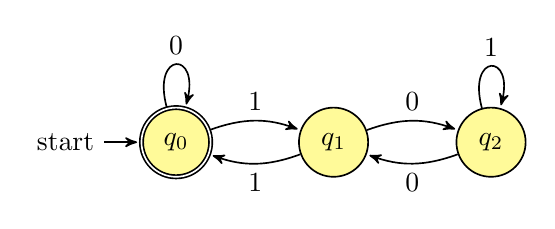
\begin{tikzpicture}[->,>=stealth',shorten >=1pt, auto, node distance=2cm, semithick]
    \tikzstyle{every state}=[text=black, fill=yellow!40]

    \node[initial,state, accepting] (q0)                    {$q_0$};
    \node[state]         (q1) [right of=q0] {$q_1$};
    \node[state]         (q2) [right of=q1] {$q_2$};

    \path (q0) edge  [loop above] node {$0$} (q0)
            edge [bend left=20] node {$1$} (q1)
        (q1) edge [bend left=20] node {$0$} (q2)
            edge [bend left=20] node {$1$} (q0)
        (q2) edge [loop above] node {$1$} (q2)
            edge [bend left=20] node {$0$} (q1)
    ;
    \end{tikzpicture}
    \end{center}
    where $Q = \{q_0, q_1, q_2\}$, $\Sigma = \{0,1\}$, and $F = \{q_0\}$. 

    \begin{enumerate}
    \item \gradeComplete Find and fix the mistake in the 
    following symbolic description of the transition function $\delta \colon Q \times \Sigma \to Q$: for each $j \in \{0,1\}$
    \[
    \delta(q_0, j) = q_j \hspace{2cm} \delta(q_1, j) = q_{1-j} \hspace{2cm} \delta(q_2, j) = q_{1+j}
    \]
    \item \gradeCorrect Keeping the same set of states $Q = \{q_0, q_1, q_2\}$, alphabet $\Sigma = \{0,1\}$, starting state $q_0$, and set
    of accepting states $F = \{q_0\}$, change the transition function $\delta$ so that the resulting finite
    automaton recognizes the language 
    described by the regular expression
    \[
        0^* \cup \Sigma^* 1000^*
    \]
    Briefly justify why the resulting finite automaton works 
    by describing the role of each state with your new transition function and relating it to a plain English description 
    of the language described by the regular expression.

    Note: with regular expressions $*$ binds more tightly than concatenation 
    so $1000^* = (100)(0^*)$.

    \end{enumerate}
    {\it (Challenge question, not graded) There is a beautiful plain English description of the language recognized by the finite automaton
    with the state diagram depicted at the start of Problem~3. 
    What is it?}

    %%%%%%%%%%% PROBLEM 4 %%%%%%%%%%%
    \item \textbf{Being precise with terminology} (5 points): \\
    For each of the following statements, determine if 
    it is true, false, or if the question doesn't even 
    make sense (because the statement isn't well formed
    or doesn't use terms in ways consistent with definitions from class).

    \begin{enumerate}
    \item\gradeComplete The empty string is in every language.
    \item\gradeComplete $\Sigma^*$ is a language.
    \item\gradeComplete Every language is a regular expression.
    \item\gradeComplete Alphabets are infinite.
    \item\gradeComplete There is a (finite) number $k \in \mathcal N$ such that every DFA has fewer than $k$ states.
    \end{enumerate}
\end{enumerate}
\newpage

\title{HW2 : Regular Languages and Automata Constructions}
\date{Due: April 18th at 5pm (no penalty late submission until 8am next morning), via Gradescope}


\maketitle
\thispagestyle{fancy}

You will practice designing multiple representations of regular languages and working with general 
constructions of automata to demonstrate the richness of the class of regular languages.

\textit{Resources}: To review the topics you are working with for this assignment, see the 
class material from Week 1 and Week 2. We will post frequently asked questions and our answers to them in a pinned Piazza post.

\textit{Reading and extra practice problems}: Sipser Section 1.1, 1.2, 1.3. 
Chapter 1 exercises 1.4, 1.5, 1.6, 1.7, 1.8, 1.9, 1.10, 1.11, 1.12, 1.14, 1.15, 1.16, 1.17, 1.19, 1.20, 1.21, 1.22.

\textit{Key Concepts:} Regular expressions, language described by a regular expression, 
deterministic finite automata (DFAs), regular languages, closure of the class of regular languages under certain operations, 
nondeterministic finite automata (NFA).

\instructions

You will submit this assignment via Gradescope
(\href{https://www.gradescope.com}{https://www.gradescope.com}) 
in the assignment called ``hw2CSE105Sp23''.

\textbf{Assigned questions}

\begin{enumerate} 

%%%%%%%%%%% PROBLEM 1 %%%%%%%%%%%

\item \textbf{It can be hard to give a good complement} (15 points): \\
For any language $L \subseteq \Sigma^*$, recall that we define its \emph{complement} as 
$$\overline{L} := \Sigma^* - L = \{w \in \Sigma^* \mid w \notin L\}$$ That is, the complement of $L$ 
contains all and only those strings which are not in $L$. Our notation for regular expressions does not 
include the complement symbol. However, 
it turns out that the complement of a language described by a regular expression is guaranteed to also be describable by a 
(different) regular expression. For example, over the alphabet $\Sigma = \{0,1\}$, the complement of the language described 
by the regular expression $\Sigma^* 0$ is described by the regular expression $\varepsilon \cup \Sigma^*1$
because any string that does not end in $0$
must either be the empty string or end in $1$.

For each of the regular expressions $R$ over the alphabet $\Sigma = \{0,1\}$ below, write the regular 
expression for~$\overline{L(R)}$. Your regular expressions may use the symbols
$\varnothing$, $\varepsilon$, $0$, $1$, and the 
following operations to combine them: union, concatenation, 
and Kleene star.

Briefly justify why your solution for each part works by giving plain English descriptions of the language 
described by the regular expression and of its complement and connecting them to the regular 
expression via relevant definitions. An English description that is more 
detailed than simply negating the description in the original language will likely be helpful in the justification.

\begin{enumerate}
    \item\gradeCorrectFirst $(\Sigma \Sigma)^*$
    \item\gradeCorrect $\Sigma^* 11 \Sigma^*$
    \item\gradeCorrect $0^* 1 0^* 1 0^*$
\end{enumerate}

%%%%%%%%%%% PROBLEM 2 %%%%%%%%%%%

\item \textbf{Closure of the class of regular languages under intersection} (12 points): \\
For this question, let $\Sigma = \{0,1\}$.
Recall the DFA over $\Sigma$ from the previous homework:
\begin{center}
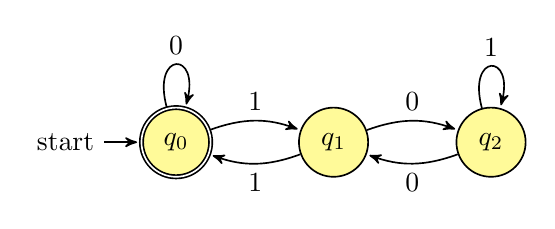
\begin{tikzpicture}[->,>=stealth',shorten >=1pt, auto, node distance=2cm, semithick]
  \tikzstyle{every state}=[text=black, fill=yellow!40]

  \node[initial,state, accepting] (q0)                    {$q_0$};
  \node[state]         (q1) [right of=q0] {$q_1$};
  \node[state]         (q2) [right of=q1] {$q_2$};

  \path (q0) edge  [loop above] node {$0$} (q0)
  		edge [bend left=20] node {$1$} (q1)
	(q1) edge [bend left=20] node {$0$} (q2)
		edge [bend left=20] node {$1$} (q0)
	(q2) edge [loop above] node {$1$} (q2)
		edge [bend left=20] node {$0$} (q1)
 ;
\end{tikzpicture}
\end{center}
We'll call the language recognized by the DFA above $A$.
Let's also define a new language $B \subseteq \Sigma^*$ to be 
the language recognized by the DFA 
over $\Sigma$ with state diagram below:
\begin{center}
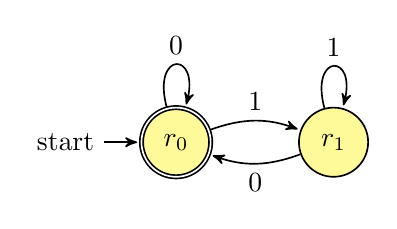
\begin{tikzpicture}[->,>=stealth',shorten >=1pt, auto, node distance=2cm, semithick]
  \tikzstyle{every state}=[text=black, fill=yellow!40]

  \node[initial,state, accepting] (q0)                    {$r_0$};
  \node[state]         (q1) [right of=q0] {$r_1$};

  \path (q0) edge  [loop above] node {$0$} (q0)
  		edge [bend left=20] node {$1$} (q1)
	(q1) edge [loop above] node {$1$} (q1)
		edge [bend left=20] node {$0$} (q0)
 ;
\end{tikzpicture}
\end{center}

\begin{enumerate}
    \item\gradeCorrect Using the construction for the intersection of two regular languages (Sipser page 46), 
    draw the state diagram for a DFA recognizing the intersection of the languages $A$ and $B$. The labels of 
    each one of your states should be the ordered pair of labels for the states from the two machines above. 
    Your diagram should have $6$ states.
    \item\gradeComplete In this part of the problem, you will prove that the general construction for the DFA 
    recognizing intersection of two languages that 
    you used in part (a) does not always produce a DFA
    with the smallest number of states possible. 
    You will do this by giving one counterexample (that combined with your work in part (a), 
    proves the general claim). Your task: design a DFA with exactly 4 states that recognizes 
    the language $A \cap B$. Briefly justify why your design works by describing the role of each state
    of your DFA and relating it to a plain English description of the language resulting from the intersection.
    \item\gradeCorrect  Later in the class we will learn that there are some languages which are not regular, 
    and in fact, we will learn specific techniques to prove that certain languages are not regular. 
    For the moment, however, we can already investigate closure properties of the class of regular 
    languages just by knowing that a non-regular language exists. 

    We know (from the textbook and our work in class) that if $L$ and $K$ are regular languages, 
    then $L \cap K$ is regular (for arbitrary languages $L$ and $K$). Prove that the converse of this statement is false; that is, 
    give a counterexample by giving a specific regular language $L$ so that
    for each non-regular language $X$, $L \cap X$ is regular (even though $X$ isn't).

    In your solution, justify why $L$ is regular 
    and why $L \cap X$ is regular (for arbitrary $X$) using relevant definitions.
\end{enumerate}


{\it (Challenge question, not graded) Prove/disprove: For 
any language $L$ over $\Sigma^*$, $L \cap B$ is regular implies $L$ is regular, where $B$ is the specific language from part (a) 
and (b) of Problem 2.}

%%%%%%%%%%% PROBLEM 3 %%%%%%%%%%%
\item {\bf Closure of the class of regular languages under} \SUBSTRING~(16 points): \\
Let $\Gamma = \{0,1,2\}$. From the previous homework, recall the function $\SUBSTRING$ that 
has domain and codomain
$\mathcal{P}(\Gamma^*)$, 
where, for each language $K$ over $\Gamma$,
$$\SUBSTRING(K) := \{ w \in \Gamma^* \mid \text{there exist } a,b \in \Gamma^* \text{ such that } awb \in K\}$$
\begin{enumerate}
\item \gradeCorrect Consider the NFA over $\Gamma$ with state diagram:
\begin{center}
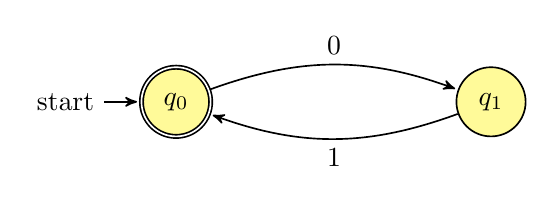
\begin{tikzpicture}[->,>=stealth',shorten >=1pt, auto, node distance=2cm, semithick]
  \tikzstyle{every state}=[text=black, fill=yellow!40]

  \node[initial,state, accepting] (q0)                    {$q_0$};
  \node		     (c)   [right of=q0] {};
  \node[state]         (q1) [right of=c] {$q_1$};
  
  \path (q0) edge [bend left=20] node {$0$} (q1)
	(q1) 	edge [bend left=20] node {$1$} (q0)
 ;
\end{tikzpicture}
\end{center}
We'll call the language recognized by the NFA above $C$.
Fill in the blanks below: 
\begin{itemize}
    \item An example of a string over $\Gamma$ that is in $C$
    {\bf and} is in $\SUBSTRING(C)$ is \underline{\phantom{\hspace{1in}}} because 
    \underline{\phantom{\hspace{1in}}}
    \item An example of a string over $\Gamma$ that is in $C$
    {\bf and} is {\bf not} in $\SUBSTRING(C)$ is \underline{\phantom{\hspace{1in}}} because 
    \underline{\phantom{\hspace{1in}}}
    \item An example of a string over $\Gamma$ that is {\bf not} in $C$
    {\bf and} is in $\SUBSTRING(C)$ is \underline{\phantom{\hspace{1in}}} because 
    \underline{\phantom{\hspace{1in}}}
    \item An example of a string over $\Gamma$ that is {\bf not} in $C$
    {\bf and} is {\bf not} in $\SUBSTRING(C)$ is \underline{\phantom{\hspace{1in}}} because 
    \underline{\phantom{\hspace{1in}}}
\end{itemize}
For each item, you'll either fill in a specific string 
and a justification that refers back to the relevant 
definitions, or you'll write ``impossible'' for the first 
part of the sentence and justify why it's impossible to find such 
an example referring back to the relevant definitions.
\item\gradeComplete Prove 
that the class of regular languages is closed under the $\SUBSTRING$ operation. Namely, give a general construction 
that takes an arbitrary NFA and constructs
 an NFA that recognizes the result of applying $\SUBSTRING$
 to the language recognized by the original machine. 
You can describe your construction in words and/or
draw a picture to illustrate your construction.
You do not have to write down a formal specification.

\item\gradeComplete Draw the state diagram of an 
NFA over $\Gamma$ that recognizes $\SUBSTRING(C)$ (for 
$C$ the language from part (a) of this Problem), using
your construction from part (b) of this Problem, or manually
constructing it. 
Describe the computation(s) of this NFA for each of the 
sample strings you gave in part (a).
\end{enumerate}

%%%%%%%%%%% PROBLEM 4 %%%%%%%%%%%
\item {\bf Closure of the class of regular star-free languages under} \REP~(7 points):\\
A language is said to be \emph{star-free} whenever it can be described by a regular expression that 
has no Kleene star operations, but where complement operation can be 
incorporated into the expression as many times as you like. 
For example, the language $$\{\varepsilon, 0010\}$$ is star-free because it can be described
by $\varepsilon \cup 0010$ which does not use the Kleene star operation symbol.
\begin{enumerate}
    \item\gradeCorrect Prove that the set of all strings 
    over $\Gamma = \{0,1,2\}$ is star-free. A complete solution
    will give an expression that describes this language 
    that does not use Kleene star but may incoporate the complement
    expression as many times as you like, along 
    with a justification that refers back to relevant definitions.
    \item\gradeComplete Prove that every finite language is star-free.
    \item\gradeComplete Let $\Sigma = \{0,1\}$. From the previous
    homework, recall the function $\REP$ that has domain 
    $\mathcal{P}(\Sigma^*)$ and codomain $\mathcal{P}(\Gamma^*)$, 
    where, for each language $L$ over $\Sigma$,
    \begin{align*}
        \REP(L) &:= \{ w \in \Gamma^* \mid \text{between every 
    pair of successive $2$'s in $w$ is a string in $L$}\}
    \end{align*}
    
    Show that $\REP(L)$ is a regular and star-free language 
    whenever $L$ is a regular and star-free language. That is, 
    given an expression $R$ describing $L$, write a regular 
    expression for $\REP(L)$ using only the regular expressions 
    $R$, $\varnothing$, $\varepsilon$, $0$, $1$, $2$, and the 
    following operations to combine them: union, concatenation, 
    and complement. You may assume that $\overline{R}$
    describes $\Sigma^* -L(R)$, that is, the complement for the regular expression $R$ over the alphabet $\Sigma$ is itself 
    a language over $\Sigma$. 
\end{enumerate}

%%%%%%%%%%% END PROBLEMS  %%%%%%%%%%%
\end{enumerate}

\newpage

\title{HW3 : Nonregular Languages and Pushdown Automata}
\date{Due: April 25th at 5pm (no penalty late submission until 8am next morning), via Gradescope}


\maketitle
\thispagestyle{fancy}

\textbf{In this assignment:}

You will practice distinguishing between regular and nonregular languages using both 
closure arguments and the pumping lemma.

\textit{Resources}: To review the topics you are working with for this assignment, 
see the class material from Week 2 through Week 4. We will post frequently asked questions 
and our answers to them in a pinned Piazza post.

\textit{Reading and extra practice problems}: Sipser Section 1.4, 2.2. Chapter 1 
exercises 1.29, 1.30. Chapter 1 problems 1.49, 1.50, 1.51.

\textit{Key Concepts:} Pumping lemma, pumping length, regular languages, nonregular languages, 
pushdown automata, stack.

\instructions

You will submit this assignment via Gradescope
(\href{https://www.gradescope.com}{https://www.gradescope.com}) 
in the assignment called ``hw3CSE105Sp23''.

\textbf{Requests from your TAs and tutors}
To help us with grading please 
\begin{itemize}
    \item Start each question on a new page.
    \item Label the start of each solution with {\bf Answer}.
\end{itemize}

\textbf{Assigned questions}

\begin{enumerate} 

%%%%%%%%%%% PROBLEM 1 %%%%%%%%%%%

\item \textbf{Regular or not?} (21 points):\\
Fix $\Sigma = \{0,1\}$ and $\Gamma = \{0,1,2\}$.
For each of the languages listed below, 
prove that it is either regular or nonregular. {\it Note:} You might find it useful to 
explore the definition of each set and 
consider alternate (simpler) ways of stating it.

For each language that is regular, a complete 
solution will include a 
precise definition of a DFA, NFA, or regular 
expression that recognizes or describes it, along 
with a brief justification
of your construction by explaining the role each 
state plays in the machine
or referring back to relevant definitions.

For each language that is nonregular, a complete
solution will use the pumping lemma to prove that it is nonregular, 
including appropriate
justification related to the specific language.

\begin{enumerate}
    \item\gradeCorrectFirst $L_1 = \{0^n x 1^n \mid n \ge 1, x \in \Sigma^*\}$, a language over $\Sigma$.
    \item\gradeCorrect $L_2 = \{0^n 1 x 0 1^n \mid n 
    \ge 1, x \in \Sigma^* \}$, a language over 
    $\Sigma$.
    \item\gradeCorrect 
    Recall that for $L \subseteq \Sigma^*$, we define
    \begin{align*}
    \REP(L) &:= \{ w \in \Gamma^* \mid \text{between every pair of successive $2$'s in $w$ is a string in $L$}\}\\
    &\phantom{:}=\{w \in \Gamma^* \mid \text{for all } v \in \Sigma^* \text{ if } 2v2 \in \SUBSTRING(\{w\})  \text{, then } v \in L\} 
    \end{align*}
    $L_3 = \REP( \{ 0^n 1^n \mid n \geq 1 \} )$, 
    a language over $\Gamma$.
\end{enumerate}


%%%%%%%%%%% PROBLEM 2 %%%%%%%%%%%

\item \textbf{Properties of nonregular languages} (21 points): \\
Prove or disprove each of the following statements. In other words, decide whether 
each statement is true or false and justify your decision. 
Let $\Sigma = \{0,1\}$ and let $\Gamma = \{0,1,2\}$.
\begin{enumerate}
    \item\gradeCorrect For all languages $L, K$ over
    $\Sigma$, if $L$ is nonregular and $K$ is finite, then $L - K$ is nonregular.
    Recall: $L - K = \{ w \in \Sigma^* \mid w \in L \text{ and } w \notin K\}$.
    \item\gradeCorrect Every infinite language over $\Sigma$ 
    where each string in the language has an equal number of $0$'s and 
    $1$'s is nonregular.
    \item\gradeCorrect Recall that for language $K$ over $\Gamma$,
    \[
    \SUBSTRING(K) := \{ w \in \Gamma^* \mid \text{there exist } a,b \in \Gamma^* \text{ such that } awb \in K\}.
    \]
    For every nonregular language $K$ over $\Gamma$, $\SUBSTRING(K)$ is nonregular.
\end{enumerate}

%%%%%%%%%%% PROBLEM 3 %%%%%%%%%%%
\item \textbf{Pumping dilemma} (8 points): \\
Your friend claims that the Pumping Lemma is useless for proving that an infinite language 
$K \subseteq \Sigma^*$ is not regular. Their logic goes like this

\begin{enumerate}[label=(Step~\arabic*), leftmargin=2cm]
\item[(Step 1)] Suppose that $K$ is regular. It can be recognized by a 
DFA $M = (Q, \Sigma, \delta, q_0, F)$.
\item[(Step 2)] For arbitrary DFA $M$, the pumping length $p$ is at least $|Q|$.
\item[(Step 3)] However, for every integer $n \ge |Q|$, there exists a machine 
$M' = (Q', \Sigma, \delta', q_0', F')$ such that $L(M') = L(M) = K$ and $|Q'| = n$.
\item[(Step 4)] Therefore, the Pumping Lemma cannot be used to pump any string 
of finite length since its pumping length might be arbitrarily large.
\end{enumerate}

Below, we will examine the steps above in detail. Justify your answer to each part.
\begin{enumerate}
    \item\gradeCompleteFirst (Step 1): Is this statement true? In other words, just because we're assuming that $K$ is regular a regular language, does it mean we can assume there is a DFA that recognizes it?

    \item\gradeComplete (Step 2): 
    In general, it's true that the smallest the pumping length of a language
    recognized by a DFA with states $Q$ can be is $|Q|$. Prove this by finding a specific infinite language $K$ and a DFA recognizing 
    where $K$ cannot have pumping length smaller than $|Q|$.

    \item\gradeComplete (Step 3): This step is correct;
    prove the stated version of this statement: For every integer $n \ge |Q|$, there 
    exists a machine $M' = (Q', \Sigma, \delta', q_0', F')$ such that $L(M') = L(M)$ and $|Q'| = n$.

    (\textit{Challenge; not graded}): 
    Define a \emph{cycle} to be a sequence of \emph{distinct} states $q_1, q_2, \ldots, q_m$ such that
	\[
	\delta(q_1, \sigma_1) = q_2, \hspace{1cm} \delta(q_2, \sigma_2) = q_3, \hspace{.5cm} \ldots, \hspace{.5cm}\delta(q_m, \sigma_m) = q_1, 
	\]
	where $\sigma_1, \sigma_2, \ldots, \sigma_m \in \Sigma$ are symbols in the alphabet. 
    An objection to the statement in (Step 3) is that the proof of the Pumping Lemma 
    depends on the length of the cycles in the DFA rather than the number of states. That is, 
    increasing the number of states in your DFA might not increase the pumping length because 
    the length of the smallest cycle stays the same. Nevertheless, a version of your friend's statement 
    is still true whenever you impose this additional cycle constraint:  for every integer $n \ge |Q|$, 
    there exists a machine $M' = (Q', \Sigma, \delta', q_0', F')$ such that $L(M') = L(M)$ and the length 
    of the smallest cycle in the $M'$ is at least $n$. \\

	Your task is to show that even this more general statement is true for the simple language $\Sigma^*$ 
    recognized by the DFA below:
	\begin{center}
    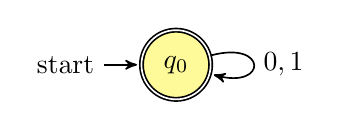
\begin{tikzpicture}[->,>=stealth',shorten >=1pt, auto, node distance=2cm, semithick]
    \tikzstyle{every state}=[text=black, fill=yellow!40]

    \node[initial,state, accepting] (q0) {$q_0$};

    \path (q0)  edge [loop right] node {$0,1$} (q0);
    \end{tikzpicture}
    \end{center}
	For all $n \ge 1$, define a DFA for this language where the length of the smallest cycle is $n$.

    \item\gradeComplete (Step 4): Describe why this statement is true/false/misleading.
\end{enumerate}


%%%%%%%%%%% END PROBLEMS  %%%%%%%%%%%
\end{enumerate}

\newpage

\title{HW4 : Pushdown Automata and Context-free grammars}
\date{Due: May 2nd at 5pm (no penalty late submission until 8am next morning), via Gradescope}


\maketitle
\thispagestyle{fancy}

\textbf{In this assignment:}

You will  practice with the definition of pushdown automata and context-free grammars and reason
about regular and context-free languages.

\textit{Resources}: To review the topics you are working with for this assignment, 
see the class material from Week 3 through Week 4. We will post frequently asked questions and 
our answers to them in a pinned Piazza post.

\textit{Reading and extra practice problems}: Sipser Sections 2.1, 2.2. 
Chapter 2 exercises 2.1, 2.2, 2.3, 2.4, 2.5, 2.6, 2.7, 2.9, 2.10, 2.11, 2.12, 2.13, 2.16, 2.17.

\textit{Key Concepts:} Pushdown automata, stack, context-free grammars, derivations, 
context-free languages.

\instructions

You will submit this assignment via Gradescope
(\href{https://www.gradescope.com}{https://www.gradescope.com}) 
in the assignment called ``hw4CSE105Sp23''.

\textbf{Requests from your TAs and tutors}
To help us with grading please 
\begin{itemize}
    \item Start each question on a new page.
    \item Label the start of each solution with {\bf Answer}.
\end{itemize}

\textbf{Assigned questions}


\begin{enumerate} 

%%%%%%%%%%% PROBLEM 1 %%%%%%%%%%%
\item \textbf{A PDA with multiple possibilities} (22 points): \\
Consider the PDA with input and stack alphabet $\Gamma = \{0,1,2\}$ whose ``unfinished" 
state diagram is given below:

\begin{center}
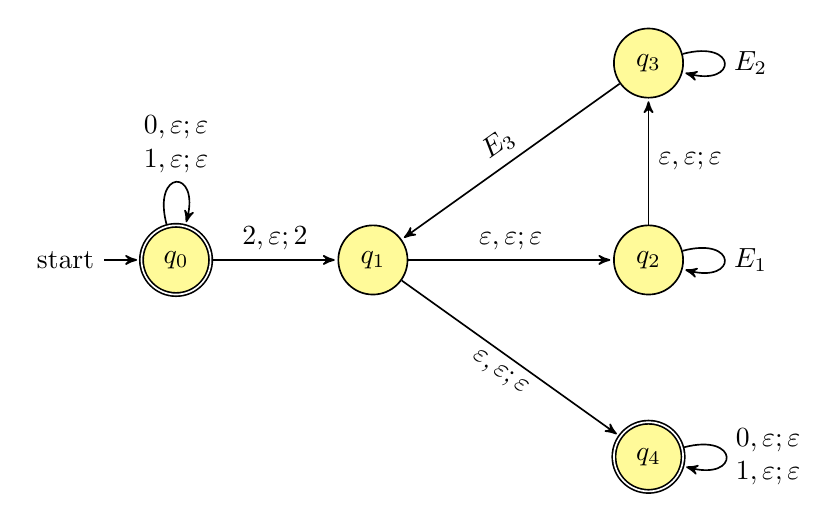
\begin{tikzpicture}[->,>=stealth',shorten >=1pt, auto, node distance=2.5cm, semithick]
  \tikzstyle{every state}=[text=black, fill=yellow!40]

  \node[initial,state, accepting] (q0)      {$q_0$};
  \node[state]         (q1) [right of=q0,  xshift=0cm] {$q_1$};
  \node[state]         (q2) [right of=q1,  xshift=1cm] {$q_2$};
  \node[state]         (q3) [above of=q2] {$q_3$};
  \node[state, accepting]         (q4) [below of=q2] {$q_4$};

  \path (q0) edge [loop above] node[align=left] {$0, \varepsilon; \varepsilon$ \\ $1, \varepsilon; \varepsilon$}  (q0)
  		edge node {$2, \varepsilon; 2$} (q1)
	(q1) 	edge node {$\varepsilon, \varepsilon; \varepsilon$} (q2)
		edge node[below, sloped] {$\varepsilon, \varepsilon; \varepsilon$} (q4)
	(q2) edge [loop right] node {$E_1$} (q2)
		edge [right] node {$\varepsilon, \varepsilon; \varepsilon$} (q3)
	(q3) edge [loop right] node {$E_2$} (q3)
		edge node[sloped] {$E_3$} (q1)
	(q4) edge [loop right] node[align=left] {$0, \varepsilon; \varepsilon$ \\ $1, \varepsilon; \varepsilon$} (q4)
 ;
\end{tikzpicture}
\end{center}

There are three labels ($E_1$, $E_2$, and $E_3$) on the edges that are unspecified. 
To be precise, each $E_i$ is of the form ``$x,y; z$'' where $x, y, z \in \Gamma_{\varepsilon}$ 
(recall $\Gamma_{\varepsilon} = \Gamma \cup \{\varepsilon\}$).

\begin{enumerate}
    \item\gradeCorrectFirst Prove that (no matter how the labels $E_1, E_2, E_3$ are specified), 
    the language recognized by this 
    PDA is infinite. A complete solution will include a precise
    description of an infinite collection of strings each 
    of which is accepted by the PDA, with 
    a precise and
    clear description of the accepting computation of the PDA on 
    each of these strings.

    \item\gradeCompleteFirst Prove/Disprove: Over all the possible choices for the labels $E_1, E_2, E_3$, 
    this PDA can only recognize finitely many languages. Justify your solution by referring back to the 
    relevant definitions.

    \item\gradeCorrect Recall that for $L \subseteq \Sigma^*$ with $\Sigma = \{0,1\}$, we define
    \begin{align*}
    \REP(L) &:= \{ w \in \Gamma^* \mid \text{between every pair of successive $2$'s in $w$ is a string in $L$}\}\\
    &\phantom{:}=\{w \in \Gamma^* \mid \text{for all } v \in \Sigma^* \text{ if } 2v2 \in \SUBSTRING(\{w\})  \text{, then } v \in L\} 
    \end{align*}
    where for all languages $K \subseteq \Gamma^*$ we let
    \[
    \SUBSTRING(K) := \{ w \in \Gamma^* \mid \text{there exist } a,b \in \Gamma^* \text{ such that } awb \in K\}.
    \]

    Determine how to set the labels $E_1, E_2, E_3$ so that the language of the PDA is 
    \[
    \REP(\{0^n1^m \mid n \ge 0, m \ge 0\})
    \]
    In addition to specifying each $E_i$, a complete justification 
    will include a precise description of why this choice of the $E_i$'s
    means that the PDA recognizes the language indicated.

    \item\gradeCorrect Determine how to set the labels $E_1, E_2, E_3$ so that the language of the PDA is 
    \[
    \REP(\{0^n1^n \mid n \ge 0\})
    \]
    In addition to specifying each $E_i$, a complete justification 
    will include a precise description of why this choice of the $E_i$'s
    means that the PDA recognizes the language indicated.
\end{enumerate}

%%%%%%%%%%% PROBLEM 2 %%%%%%%%%%%
\item \textbf{Grammar practice} (12 points): \\
For each of the languages listed below, 
define a context-free grammar 
$G = (V, \Sigma, R, S)$ that generates the 
language. Instead of formally justifying
your grammar, illustrate it by giving 
{\bf two examples} 
of strings in the language 
and their derivations using your grammar
and {\bf one example} of a string not
in the language with an explanation
of why it cannot appear 
on the right side of any derivation 
in your grammar. Choose your
examples so they are different enough 
to illustrate the role of 
as many of the variables 
in your grammar as possible.

\begin{enumerate}
    \item\gradeCorrect $\REP(\{0^n1^n \mid n \ge 0\})$

    \item\gradeCorrect $\{1^n = 1^a + 1^b \in \{1,=,+\}^* \mid a,b,n \ge 1 \text{ such that } a + b = n \}$
\end{enumerate}

%%%%%%%%%%% PROBLEM 3 %%%%%%%%%%%
\item \textbf{Substrings and regularity} (16 points): \\
For this problem, we fix the 
alphabet $\Gamma = \{0,1,2\}$. Recall the 
definition of the function $\SUBSTRING$ from 
Problem 1.
\begin{enumerate}
\item\gradeCorrect Prove that $\SUBSTRING(\{ 0^n 1^n \mid n \ge 0\})$ is regular.
A complete 
solution will include a 
precise definition of a DFA, NFA, or regular 
expression that recognizes or describes it, along 
with a brief justification
of your construction by explaining the role each 
state plays in the machine
and referring back to relevant definitions.
\item\gradeCorrect Prove that 
$\SUBSTRING(\{ 0^n 1^n 2^n \mid n \ge 0\})$
is not regular.
\item\gradeComplete Is  $\SUBSTRING(\{ 0^n 1^n 2^n \mid n \ge 0\})$
context-free?
Informally justify your answer, referring 
to class discussions and/or the textbook.

\end{enumerate}
%%%%%%%%%%% END PROBLEMS  %%%%%%%%%%%
\end{enumerate}

\newpage

\newcommand{\blank}{\scalebox{1.5}{\textvisiblespace}}
\newcommand{\corrupted}{\text{\lightning}}

\title{HW5 : Turing Machines}
\date{Due: May 16th at 5pm (no penalty late submission until 8am next morning), via Gradescope}


\maketitle
\thispagestyle{fancy}

\textbf{In this assignment:} You will practice designing and working with Turing machines and their variants.

\textit{Resources}: To review the topics you are working with for this assignment, 
see the class material from Week 5 through Week 6. We will post frequently asked questions 
and our answers to them in a pinned Piazza post.

\textit{Reading and extra practice problems}: Chapter 3. Chapter 3 exercises 3.1, 3.2. 

\textit{Key Concepts:} Formal definitions of Turing machines, computations of Turing machines, 
halting computations, implementation-level descriptions of Turing machines, high-level descriptions 
of Turing machines, recognizable languages, decidable languages, variants of Turing machines, 
enumerators, nondeterministic Turing machines, Church-Turing thesis.

\instructions

You will submit this assignment via Gradescope
(\href{https://www.gradescope.com}{https://www.gradescope.com}) 
in the assignment called ``hw5CSE105Sp23''.

\textbf{Assigned questions}

\begin{enumerate} 
%%%%%%%%%%% PROBLEM 1 %%%%%%%%%%%

\item $\REP$(\textbf{Describing a Turing Machine for }$\REP$) 
(18 points): \\
Recall that for $L \subseteq \Sigma^*$ with $\Sigma = \{0,1\}$, 
we define the language over $\Gamma = \{0,1,2\}$
\begin{align*}
\REP(L) &:= \{ w \in \Gamma^* \mid \text{between every pair of successive $2$'s in $w$ is a string in $L$}\}\\
&\phantom{:}=\{w \in \Gamma^* \mid \text{for all } v \in \Sigma^* \text{ if } 2v2 \in \SUBSTRING(\{w\})  
\text{, then } v \in L\} 
\end{align*}
where for all languages $K \subseteq \Gamma^*$ we let
\[
\SUBSTRING(K) := \{ w \in \Gamma^* \mid \text{there exist } a,b \in \Gamma^* \text{ such that } awb \in K\}.
\]

In this question, you will give three separate descriptions of a Turing machine 
which recognizes the language $\REP(\{0^n1^n \mid n \ge 0\})$. 

This may seem like a somewhat tedious process, but we think that it is important 
to see all the different descriptions in action at least once for a single language.

With each description, give a brief justification connecting the description to the language it recognizes.

\begin{enumerate}
\item\gradeCompleteFirst High-level description: 
description of algorithm (precise sequence of instructions), 
without implementation details of machine. Your description 
can use data structures and refer to specific positions 
in the input strings (without specifying memory management).

\item\gradeCorrectFirst Implementation-level description: English prose that 
describes the Turing machine head movements relative to contents of tape, 
and conditions for accepting / rejecting based on those contents.

\item\gradeCorrect Formal definition: Give the 7-tuple of parameters 
$$(Q, \Sigma, \Gamma, \delta, q_0, q_{\mathrm{acc}}, q_{\mathrm{rej}})$$ 
describing the Turing Machine. Represent the transition 
function $\delta$ by drawing the
state diagram of the Turing machine. You may use the following 
conventions: omit the reject state from the diagram; any missing 
transitions in the state diagram are assumed to go to the reject state.

\end{enumerate}

%%%%%%%%%%% PROBLEM 2 %%%%%%%%%%%

\item \textbf{This Turing Machine is broken... or is it?} 
(12 points): \\
Let's consider a variant of a Turing Machine which models computation 
where the data keeps getting corrupted. A Corrupted Turing Machine $M = 
(Q, \Sigma, \Gamma, \delta, q_0, q_{\mathrm{acc}}, q_{\mathrm{rej}})$ has 
some of the usual Turing Machine components: set of states ($Q$); input 
alphabet ($\Sigma$); transition function ($\delta$); start state ($q_0$); 
accepting state ($q_{\mathrm{acc}}$), rejecting state 
($q_{\mathrm{rej}}$). Unlike a normal Turing Machine, the tape alphabet 
$\Gamma  \supseteq \Sigma$ has two (rather than one) special characters $\blank$ and $\corrupted$:
\begin{itemize}
\item $\blank \in \Gamma$, $\blank \not\in \Sigma$: This is the usual blank symbol. 
\item $\corrupted \in \Gamma$, $\corrupted \not\in \Sigma$: This symbol indicates a cell that 
has been corrupted. The machine cannot write over any corrupted cell; that is, for each $q \in Q$,
\[
\delta(q, \corrupted) \in \{ (r, \corrupted, D) \mid r \in Q, D \in \{L, R\} \}
\]
\end{itemize} 

Computation in the corrupted Turing Machine proceeds as normal except that sometimes when 
writing a tape symbol as intended, a $\corrupted$ symbol is written instead. Thankfully, 
the pattern of corruption is predictable: the first write is corrupted, and then every 
other write thereafter is corrupted. That is, the first, third, fifth,... etc.\ writes are corrupted.

\begin{enumerate}
\item\gradeCorrect Prove that for every {\bf regular} language $L$, there exists a corrupted 
Turing Machine $M$ that recognizes $L$.

\item\gradeComplete It will turn out that the Corrupted Turing Machine is no less powerful than our 
usual definition of a Turing Machine. Let's break the proof into a few steps. First, define the 
alphabet $\Sigma_{\mathrm{pairs}}:= \Sigma \times \Sigma = \{ (a,b) \mid a \in \Sigma, b \in \Sigma\}$ 
of pairs of symbols in $\Sigma$. Give the construction of a Corrupted Turing Machine that takes 
input $a = a_1 a_2 \cdots a_n \in \Sigma^*$ and rewrites it as pairs of symbols interspersed 
by corrupted symbols. To be precise, the Corrupted Turing Machine should take starting tape configuration
\[
\begin{array}{| c | c | c | c | c | c | c | c | }  \hline
a_1 & a_2 & \ldots & a_{n-1} & a_{n} & \blank & \blank & \ldots \\ \hline
\end{array}
\]
to the tape configuration 
\[
\begin{array}{| c | c | c | c | c | c | c | c | c | c | c | c| }  \hline
\corrupted & (a_1, a_2) & \corrupted & (a_3,a_4) & \corrupted & \ldots& \corrupted 
& (a_{n-1}, a_{n}) & \corrupted & \blank & \blank & \ldots \\ \hline
\end{array}
\]
with the head once again pointing to the first cell. For simplicity, you may assume that $n$ is even.

\item\gradeComplete Starting from the tape configuration we created in the previous step, 
describe the implementation of a Corrupted Turing Machine which simulates the computation of 
any normal/uncorrupted Turing Machine.

\vspace{1em}
\noindent\textit{Challenge; not graded}: A key idea in the construction above was 
to increase the number of symbols in our tape alphabet. Can you do the same construction 
\emph{without} increasing the size of the tape alphabet? That is, for every language $L$ 
recognized by a normal Turing machine over alphabet $\Sigma$ and tape alphabet $\Sigma \cup \{\blank\}$, 
is there a Corrupted Turing Machine with tape alphabet $\Sigma \cup \{\blank,\corrupted\}$ that recognizes $L$?

\end{enumerate}

%%%%%%%%%%% PROBLEM 3 %%%%%%%%%%%

\item \textbf{True/False enumerator} (20 points): \\
For each of the following statements, determine if it is true or false. 
Clearly label your choice 
by starting your solution with {\bf True} or {\bf False} and then
provide a brief (3-4 sentences or so) justification for your answer.
\begin{enumerate}
\item\gradeCorrect Every enumerator enumerates an infinite language.
\item\gradeCorrect Let $E$ be any enumerator and $M$ be any Turing machine.
If $L(E) = L(M)$, then $M$ enters the reject state for all strings not in $L(E)$.
\item\gradeCorrect Let $E$ be any enumerator over $\Sigma$.
Suppose $a, b \in \Sigma^*$ and $a, b \in L(E)$.
If $E$ prints $a$ before $b$, then $|a| \le |b|$.
\item\gradeCorrect Let $M$ decide language $L$ over $\Sigma$
such that $M$ halts on all inputs $w \in \Sigma^*$ in $|w|^{2023}$ steps. 
There exists an enumerator $E$ with the following properties: $L(E) = L(M)$; 
and if $a, b \in L$ and $|a| < |b|$, then $E$ prints $a$ before $b$.
\item\gradeCorrect Let $N$ be a nondeterministic Turing machine. 
There is an enumerator $E$ that enumerates the set of all and only 
strings accepted by $N$ that have odd length.

\end{enumerate}

%%%%%%%%%%% END PROBLEMS  %%%%%%%%%%%
\end{enumerate}

\newpage

\title{HW6 : Computational Problems, Recognizability, Decidability}
\date{Due: May 23th at 5pm (no penalty late submission until 8am next morning), via Gradescope}


\maketitle
\thispagestyle{fancy}

\textbf{In this assignment:} You will use general constructions and specific machines 
to explore the classes of recognizable and decidable languages. You will explore various 
ways to encode machines as strings so that computational problems can be recognized.

\textit{Resources}:  To review the topics you are working with for this assignment, 
see the class material from Week 6 through Week 7. We will post frequently asked questions 
and our answers to them in a pinned Piazza post.

\textit{Reading and extra practice problems}: Chapter 4 exercises 4.1, 4.3, 4.4., 4.5. 
Chapter 4 Problems 4.29, 4.30.

\textit{Key Concepts:} uring-recognizable languages, Turing-decidable languages, 
Church-Turing thesis, computational problems.

\instructions

You will submit this assignment via Gradescope
(\href{https://www.gradescope.com}{https://www.gradescope.com}) 
in the assignment called ``hw6CSE105Sp23''.

\textbf{Assigned questions}

\begin{enumerate} 
%%%%%%%%%%% PROBLEM 1 %%%%%%%%%%%
\item \textbf{Explicit encodings} (8 points): \\
In a computational problem, the elements of the language are encodings of machines. For example, 
consider the language 
\[
E_{\mathrm{DFA}} := \{ \langle M \rangle \mid M \text{ is a DFA, and } L(M) = \varnothing \}
\]
where each string $\langle M \rangle$ in the language encodes a DFA $M = (Q, \Sigma, \delta, q_0, F)$.
Usually, we purposefully drop the details about how this encoding is done because they can distract from 
the central computational 
properties of the language. In fact, any encoding can be used so long as there exists a decider for 
syntactic questions about the DFAs being encoded. 
In this question, we will build some specific 
explicit examples of encodings of DFAs to get more comfortable with these ideas.

\begin{enumerate}
\item\gradeCompleteFirst \textit{Encoding with delimiters:} Perhaps the most straightforward
way to create an encoding is to have it mirror the structure of the tuple $(Q, \Sigma, \delta, q_0, F)$ 
for the DFA. Your task: describe an encoding that maps each DFA $M$ to a distinct string $\langle M \rangle$ 
that uniquely identifies $M$. That is, if you ``decode'' the encoding, you get the exact same machine back. 

\noindent{\it Hints, tips, notes of caution:}
\begin{itemize}[itemsep=-10pt]
\item You may use special characters like $\#$ and $\$$ as delimiters in your encoding to separate the 
various components. \\
\item Your encoding alphabet must be finite
\end{itemize}
\item\gradeComplete Use your encoding from part (a) to produce
the string encoding the DFA below:
\begin{center}
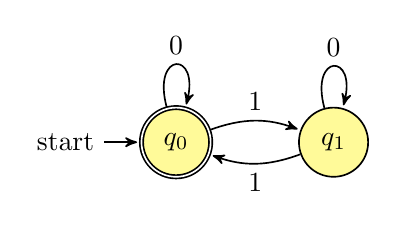
\begin{tikzpicture}[->,>=stealth',shorten >=1pt, auto, node distance=2cm, semithick]
  \tikzstyle{every state}=[text=black, fill=yellow!40]

  \node[initial,state, accepting] (q0)                    {$q_0$};
  \node[state]         (q1) [right of=q0] {$q_1$};

  \path (q0) edge  [loop above] node {$0$} (q0)
  		edge [bend left=20] node {$1$} (q1)
	(q1) edge [loop above] node {$0$} (q1)
		edge [bend left=20] node {$1$} (q0)
 ;
\end{tikzpicture}
\end{center}

\item\gradeComplete Show that it is possible to have the same kind of delimited encoding without 
using special delimiter characters. In particular, prove that for every DFA $M$, 
we can assume that $\langle M \rangle \subseteq \{0,1\}^*$.

\end{enumerate}

\noindent\textit{Challenge; not graded:\newline For the delimited encoding schemes above, 
there are strings over the encoding alphabet 
($\Sigma$) that nevertheless do not correspond to a valid DFA. \newline \newline
Prove/disprove: There exists an encoding scheme for which this is not true; that is, 
\[\{ \langle M \rangle \mid M \text{ is a DFA}\} = \Sigma^*.\]}

\vfill

%%%%%%%%%%% PROBLEM 2 %%%%%%%%%%%

\item \textbf{Closure} (18 points): \\
Let $\Sigma = \{0,1\}$ and $\Gamma = \{0,1,2\}$. Recall the functions
    \begin{align*}
    \SUBSTRING(K) &:= \{ w \in \Gamma^* \mid \text{there exist } a,b \in \Gamma^* \text{ such that } awb \in K\} \\
    \REP(L) &:= \{ w \in \Gamma^* \mid \text{between every 
    pair of successive $2$s in $w$ is a string in $L$}\}\\
    &\phantom{:}=\{w \in \Gamma^* \mid \text{for all } v \in \Sigma^* \text{ if } 2v2 \in \SUBSTRING(\{w\})  \text{, then } v \in L\}
    \end{align*}
\begin{enumerate}
    \item\gradeCorrectFirst Prove that, given any deterministic decider
    over $\Sigma$, $M_L$, there is a deterministic decider over 
    $\Gamma$ that recognizes $$\REP(~L(M_L)~)$$
    In other words, you 
    will prove that for any Turing-decidable language $L$ over $\Sigma$, 
    $\REP(L)$
    is also Turing-decidable. A complete answer will 
    include both a precise construction of the machine and a 
    (brief) justification of why this machine works as required.
    
    \item\gradeCorrect Prove that, given any nondeterministic Turing machine over 
    $\Gamma$, $N_L$, there is a nondeterministic Turing machine over 
    $\Gamma$ that recognizes $$\SUBSTRING(~L(N_L)~)$$
    In other words, you will prove that the class of Turing-recognizable languages 
    over $\Gamma$ is closed 
    under the $\SUBSTRING$ operation.
     A complete answer will 
    include both a precise construction of the machine and a 
    (brief) justification of why this machine works as required.
    
    \item\gradeComplete Give a different proof that the class of Turing-recognizable 
    languages over $\Gamma$ is closed 
    under the $\SUBSTRING$ operation, this time using only deterministic Turing machines.  A complete answer will 
    include both a precise construction of the machine and a 
    (brief) justification of why this machine works as required.

\end{enumerate}


%%%%%%%%%%% PROBLEM 3 %%%%%%%%%%%
\item \textbf{Computational problems} (24 points): \\
For each of the following statements, determine if it is true or false. 
Clearly label your choice 
by starting your solution with {\bf True} or {\bf False} and then
provide a brief (3-4 sentences or so) justification for your answer.

\begin{enumerate}
\item\gradeCorrect For each regular language $K$, the language 
\[
\{ \langle M \rangle \mid M \text{ is a DFA and } L(M) = K\} 
\]
is decidable.

\item\gradeCorrect For each regular language $L$, the language
\[
\{ \langle M_1, M_2 \rangle \mid M_1, M_2\text{ are both DFA and } 
L(M_1) \subseteq L \text{ and } L(M_2) \subseteq \overline{L}\}
\]
is decidable.


\item\gradeCorrect Let $\mathrm{Model} \in \{\mathrm{DFA}, \mathrm{NFA}, 
\mathrm{REX}, \mathrm{CFG}, \mathrm{PDA} \}$. If $EQ_{\mathrm{Model}}$ is decidable, 
then $E_{\mathrm{Model}}$ is decidable.

\end{enumerate}

{\it Challenge; not graded: Let $\mathrm{Model} \in \{\mathrm{DFA}, \mathrm{NFA}, 
\mathrm{REX}, \mathrm{CFG}, \mathrm{PDA} \}$. If $A_{\mathrm{Model}}$ is decidable, 
then $EQ_{\mathrm{Model}}$ is decidable.}

%%%%%%%%%%% END PROBLEMS  %%%%%%%%%%%
\end{enumerate}

\newpage
\titleformat{\subsubsection}[runin]
   {\normalfont\bfseries}{}{}{}
   
\title{Project - CSE 105 Spring 2022}
\date{Due 6/1/23 at 5pm (no penalty late submission until 8am next day)}


\maketitle

\thispagestyle{fancy}

The project component is designed for you to go deeper and extend your work on assignments 
and to explore an application of your choosing. 
The project is an individual assignment and has 
two tasks: 
\begin{itemize}
    \item Task 1: A meaningful language (written) and \item Task 2: A helpful function (some programming, presented as a screencast video).
\end{itemize}
\vspace{-20pt}


\subsubsection*{What resources can you use?}
This project must be completed individually, without any help from other people, 
including the course staff (other than logistics support if you get stuck with screencast). 

You can use any of this quarter's CSE 105 offering (notes, readings, class videos, homework feedback). 
These resources should be more than enough. 

If you are struggling to get started and want to 
look elsewhere online, you must acknowledge this by listing and 
citing any resources you consult 
(even if you do not explicitly quote them), including any large-language model style resources. 
Link directly to them and include the name of the 
author / video creator, any search strings or prompts you used, and the reason you consulted this reference. 

The work you submit for 
the project needs to be your own. Again, you shouldn't need to look anywhere other 
than this quarter's material and doing so may result in definitions or notations 
that conflict with our norms in this class so think carefully before you go down this path.

\subsubsection*{Submitting the project}
You will submit a PDF for Task 1 and a video for Task 2 
to an online assignment on Gradescope.

\newpage
\subsection*{Task 1: A meaningful language}

Automaton models are useful for concisely representing patterns. 
In this question, you'll choose a pattern in an application you care about, 
define it precisely, and then build a DFA, NFA, or PDA that 
recognizes it.

First, pick {\bf one} application for your example. 
Here are some ideas to 
get you started - but you can choose to go in a different direction all together.
\begin{itemize}
\item Data validation for input in text files (e.g. emails with 
specific domains, dates in specific formats, PIDs in a class list, etc.)
\item Finding ASCII codes for punctuation in a binary file.
\item The CDC recommended procedure for hand washing (Refer to the guidelines from the CDC here https://www.cdc.gov/handwashing/index.html in your explanation. You might find the first example in chapter 1 about automatic door controllers helpful when starting your design.)
\item See more ideas here: 

{\scriptsize \url{https://theory-cs.github.io/files/practical-applications-of-theory-of-computation.pdf}}
\end{itemize}

Then:
\begin{enumerate}
    \item In a paragraph or so, give the context for your chosen
    application and why you chose it.
    \item Specify the alphabet for your example.
    \item Write a precise (mathematical and/or English) description
    of a set of strings over this alphabet that is important, 
    and include a sentence or so justifying why this set is important.
    \item Give one example of a string in this set and a string not 
    in this set, and explain why you chose these example strings.
    \item Classify your language as regular or context-free, and prove
    this classification by giving an appropriate machine that
    recognizes your language. Justify your construction.
\end{enumerate}

\subsubsection*{Grading criteria and checklists}

Solution is typed out in detail step-by-step, with clear and 
correct logic and justification.

Each of the five items are included, with precise language and notation
for all terms and complete, correct, and clear justification.

\newpage
\subsection*{Task 2: A helpful function}

To relate the difficulty level of one language to another 
we use mapping reduction, which relies
on the notion of computable function. In this part of the project, 
you will define, program, and trace a specific 
computable function from $\{a,b\}^*$ to $\{a,b\}^*$.

First, choose a function you will be working with. You can pick any function you like so long as:
	\begin{itemize}
		\item Its domain is $\{a,b\}^*$ and its 
                codomain is $\{a,b\}^*$
		\item There is at least one domain 
                element that is mapped to a string that is 
                {\bf longer} than it and there is at least one 
                domain element that is mapped to a string that is 
                {\bf shorter} than it.
	\end{itemize}
Then:
 \begin{enumerate}
    \item Give a high-level description of a Turing machine that computes
    this function.
    \item Draw the state diagram of this Turing machine.
    \item Write a program in Java, Python, JavaScript, or C++ (or 
        another programming language of your choosing)
        that simulates the computations of this Turing machine.
        Your program should display a snapshot of each step of the computation, 
        including the state of the machine, the current (non-blank)
        contents of the tape, and the location of the read/write head
        of the Turing machine. If you would like, you may 
        use aids such as co-pilot or ChatGPT to help you write this 
        program. However, you should test the code that is 
        produced and be able 
        to explain what it is doing. As a header in 
        your code file, include a comment block describing 
        any resources that were used to help
        generate your code.
    \item Run your program on a string over $\{a,b\}$ which 
        the function maps to a string that is longer than it, and
    \item Run your program on a string over $\{a,b\}$ which 
        the function maps to a string that is shorter than it.
\end{enumerate}

 Presenting your reasoning and demonstrating it via screenshare are important skills that 
 also show us a lot of your learning. Getting practice with this style of presentation is a 
 good thing for you to learn in general and a rich way for us to assess your skills. To demonstrate your work, you will create 
 a 3-5 minute screencast video with the following components:
 \begin{itemize}
	\item Start with your face and your student ID for a 
        few seconds at the beginning, and introduce yourself audibly 
        while on screen. 
	You don't have to be on camera for the rest of the 
        video, though it's fine if you are. 
	We are looking for a brief confirmation that it's 
        you creating the video and 
	doing the work you submitted.
	\item Present the function you will be working with.
	Your video should include a clear and precise definition of the               function (before you introduce any Turing machines).
	\item Show on the screen and explain the high-level description of
        your Turing machine witnessing that your function is computable.
	\item Show on the screen and explain the state diagram of 
        your Turing machine.
	\item Show on the screen and present your code, including
        the software design choices you made (e.g.\ which data structures
        are you using, etc.) and any resources you used.
        \item Demonstrate running your code on the two 
        example input strings specified above. Explain why the output 
        of your program is what you would expect.
\end{itemize}


\subsubsection*{Grading criteria and checklists}

Logistics: video loads correctly, is between 3 and 5 minutes, 
shows the student's face and ID, and they introduce themself 
audibly while on screen.

The video clearly states which function was chosen for study, 
the function which is well-defined and computable, the video
presents the two different descriptions of the Turing machine clearly,
and the Turing machine correctly computes the function.

The video clearly describes which programming language was chosen 
for the implementation and gives the reasons why.

The video discusses the connections between the state diagram of the 
Turing machine
and its implementation in the code.

The video clearly demonstrates all test cases, including both expected
and actual output. The video should include screencasts of 
running the code live to demonstrate these test cases.


\subsubsection*{Your video:} You may produce screencasts 
with any software you choose. 
One option is to record yourself with Zoom; a tutorial on how to use 
Zoom to record a 
screencast (courtesy of Prof. Joe Politz)  is here: 

\url{https://drive.google.com/open?id=1KROMAQuTCk40zwrEFotlYSJJQdcG_GUU}.

The video that was produced from that recording session in Zoom is here:

\url{https://drive.google.com/open?id=1MxJN6CQcXqIbOekDYMxjh7mTt1TyRVMl}

Please send an email to the instructors 
(minnes@ucsd.edu and 
dgrier@ucsd.edu) if you have 
concerns about  the video / screencast components of this project or 
cannot complete projects in this style for some reason.

\newpage

\end{document}